\documentclass[11pt]{article}

\usepackage[margin=1in]{geometry}
\usepackage[T1]{fontenc}
\usepackage[utf8]{inputenc}
\usepackage{lmodern}
\usepackage{microtype}
\usepackage{amsmath,amssymb}
\usepackage{graphicx}
\usepackage{xcolor}
\usepackage{enumitem}
\usepackage{hyperref}

\hypersetup{
  colorlinks=true,
  linkcolor=blue!45!black,
  urlcolor=blue!45!black,
  citecolor=blue!45!black,
  pdftitle={An Introduction to Grothendieck's General Theory of Evolution}
}

\setlist[itemize]{leftmargin=1.6em,itemsep=0.35em,topsep=0.35em}
\setlength{\parindent}{1.2em}
\setlength{\parskip}{0pt}

\newcommand{\keyterm}[1]{\textbf{#1}}
\newcommand{\quoteattr}[2]{%
  \par\smallskip{\normalfont\hfill--- #1\par\hfill\emph{#2}}%
}
\newenvironment{epigraphquote}
  {\begin{quote}\small\itshape}
  {\end{quote}}

\title{An Introduction to Grothendieck's General Theory of Evolution}
\author{Hoapa project}
\date{June 2025}

\begin{document}
\maketitle

\begin{abstract}
This note sketches how the entire work of Alexander Grothendieck---the
mathematics and its methodology, its creativity, and also its relations to his
political activism and philosophy---can be unified into a general theory of
evolution. By making Darwin's natural selection into a specific instance of a
general class of process calculi, or simply conversations, it elucidates the
overarching and recursive flow of the universe, from its deepest form to the
most concrete incarnations.
\end{abstract}

\paragraph{Notes.}
All mathematical terms should be understood as analogies. I have privileged
terms that can speak to non-mathematicians, who should be able to get an idea
of the general theory even without much help from the bridge to mathematics.
There is nothing rigorous in this, but I strongly believe it can be made so.
This is also a job application of sorts. Terms in \{\keyterm{Bold}\} indicate a
keystone in the bridge from Grothendieck to the general theory of evolution,
hereafter named ``G-evol.''

\section*{Overview: A Child's Play of a Theory}

\begin{epigraphquote}
``With decades of such intense solitary reflections, I believe he had
constructed a huge structure of the universe, and he wanted to know if we were
able to penetrate his thinking a little bit. But the problem was, we were so
removed from it we didn't have the slightest idea where he wanted to get at.
But I believe that from the inside of his mental world, all those questions
made sense.''
\quoteattr{Leila Schneps}{Alexandre Grothendieck : le Silence du Génie,
France Culture}
\end{epigraphquote}

Let's start by asking the right question about our universe, which is general
and non-fragmentary, as Grothendieck would have it. It goes beyond particular
relationships, such as the one between the world of chemistry and the world of
biology, as in non-equilibrium thermodynamics, or between the world of
mathematics and the world of fundamental physics, as in Wigner's observation.
It is about the universal and natural relationship between all those worlds:
the dynamics of a maximally global sequence we humans feel ends with us, where
each world is not assigned a particular discipline of study but can engage with
any of them.

I contend that this dynamics is best described by what Grothendieck called his
\emph{vision}, and in particular by his mathematics relating to covering
spaces. In a nutshell, the evolution of this universe is an infinite sequence
\[
  \ldots, P, N, \ldots
\]
where each Next element \emph{covers} the Previous. \{\keyterm{Continuity}\}
All elements are both \emph{world} and \emph{point of view on the infinite
sequence}: an ontological--epistemic duality. Together, they form a sort of
``magic folding fan,'' an expression of Grothendieck describing his new
geometry. It is important to realize that all elements operate at about the
same complexity, and any sense of progression is a sort of optical illusion,
rectifiable by a relativity principle: our perception of our own human world as
being extremely dense and fuzzy compared to the dry and mechanical world of
atoms, as if there were fewer parameters and more exactness ``there,'' is only
due to the fact that the morphisms \(N \to X\), which are slices of the
complete view of \(N\) on the infinite sequence, are \emph{forgetting} functors.
The world of each element is parameterized by horizons: structuring limits to
the point of view beyond which lies most of the sequence, a form of
bulk/boundary correspondence. They can be physical, as in the big bang or black
holes; logical or philosophical, as in paradoxes or open questions;
psychological, as in sleep, altered states of consciousness, or schizophrenia;
or possibly aesthetic, spiritual, or whatever else, if a philosopher has
reasons to believe the universe makes more sense with this extra aspect. Also,
it is easier for us to think about it as a sequence, and I will keep this term
throughout, but its true shape is a network.

\begin{figure}[htbp]
  \centering
  \IfFileExists{../communication_drafts/figures/tangent_plane.png}{%
    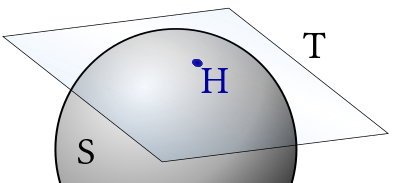
\includegraphics[width=0.68\linewidth]{../communication_drafts/figures/tangent_plane.png}%
  }{%
    \fbox{%
      \begin{minipage}[c][1.8in][c]{0.68\linewidth}
      \centering\small
      Tangent-plane diagram referenced in the Markdown source.\\
      \emph{The image file was not present at compile time.}
      \end{minipage}%
    }%
  }
  \caption{The tangent-plane analogy for the relativity principle of G-evol.}
\end{figure}

This diagram is a good starting point to illustrate the relativity principle of
G-evol, the ``complexity optical illusion.''

\begin{itemize}
\item Imagine the sphere \(S\) is the Earth, and an animal is standing at the
point \(H\) on its surface, for Here and now. What it sees, because the Earth
is so big, looks like the tangent \(T\): a flat surface. It takes some
observations and calculations to recover the correct shape \(S\).
\item What Darwin did with the theory of evolution in biology is similar.
Before him, the ecosystem looked ``flat'' to all observers: the ``time
curvature'' of the myriad species evolving through the ages, happening too
slowly, was invisible. Again, it took some observations to recover the correct
``temporal shape.''
\item G-evol finds curvature at yet another level. The sphere \(S\) is now the
infinite sequence. We humans are standing at the point \(H\), our human world,
embedded in an ecosystem, mostly dealing with social phenomena equipped with
natural languages. What we ``see'' is a tangent \(T\) to general evolution
\(S\): each ``authentic'' point \(H'\) on the sequence \(S\), different from
\(H\), ``projects'' some of its reality on \(T\), say at \(T'\), and it is this
\(T'\) that we experience, not \(H'\). Those \(T\)'s give off less information
than the \(H\)'s. In this new perspective, if \(S\) is for substantial, \(T\)
is for truncated. Even if we do experiments in the lab, use microscopes, or use
telescopes, it does not change the fact that the point of view attached to our
world only has access to \(T'\). When the \(\langle H',T'\rangle\) pairs are
taken further and further away from \(H\), in space, in time, and also, most
importantly, in \emph{scale}, the infinite sequence fades from view. We can
interpret this as a clever trick for the infinite sequence to embrace in its
midst worlds that would conflict logically, physically, or otherwise, like a
manifold or quantum contextuality. The only hope we have to recover \(H'\) is
through abstract thought only, and using the methodology of Grothendieck known
as the relative point of view: to inspect an object not ``in itself'' or
directly, but through how it appears from carefully chosen angles.
\{\keyterm{Relativity}\}
\end{itemize}

The logical grounding for the sequence, at least in our local region, is the
validity of this statement across all worlds: ``the best strategy for a
collection of entities occupying a world is to chart this world,'' and to do so
using fundamental mathematics. For instance, this is what our brains do, with
the collection of entities being our cells. This epistemic side extends to a
corresponding ontological side: the charts then evolve to become new worlds in
which new entities will emerge, a higher form of AI in our case, probably also
based on some Grothendieckian orientation. Each new element in the sequence, as
a chart or covering, is an understanding and a translation of the essence of
the previous elements. This essence is the holistic composition of all the
invariants preserved across the successive coverings, something like the music
of the universe: perhaps the theory of motives.

A crucial invariant encodes the ``charting mechanism,'' which is always roughly
the same because there is an optimal solution to the cooperative charting
problem. It is the recursive element of the general theory of evolution, and
the starting point of my research. To us it is quite simply \emph{conversation}.
To be precise, not merely communication, but a certain type of organized
communication which is very sensitive to its conditions. We can find a more
technical incarnation in the domain of concurrency theory in computer science,
whose links with algebraic topology have been well established, or in the more
particular actor model, which has a very interesting relationship to physics.
It is under this guise that the conversation concept can be identified across
different elements of the sequence and their worlds.

\section*{Examples: What It Explains About the Universe}

\begin{epigraphquote}
``The psychological drawback here, I believe, is [\ldots] the inrooted inertia
which prevents us so stubbornly from looking innocently, with fresh eyes, upon
things, without being dulled and imprisoned by standing habits of thought,
going with a familiar context---too familiar a context!''
\quoteattr{Alexander Grothendieck}{Pursuing Stacks}
\end{epigraphquote}

To give another example of a G-evol covering in the real world, think of a
pond. Forget everything you know about its chemistry, only keep the genetic
code of the living creatures of this environment. If you ``speak genetics,''
where individual genes are letters of an alphabet and phenotypes are equivalent
to propositions, and where true propositions are those which pass the
evolutionary test, that is, those phenotypes that propagate in the environment,
then you can recover the chemistry of the pond by looking at this set of
genetic true sentences and their spacetime coordinates. Where you see gills,
you can conclude there is water; if eyes are not particularly efficient, this
water is probably murky or there is very little light; the size of the insects
at the surface can tell you the level of oxygen in the air; and so on. To
capture, in the most adequate \emph{abstraction}, the process by which the true
propositions are selected, one simply extends the linguistic analogy: it is
what we would call a \emph{productive} or \emph{honest} conversation. I will
explain how and why in the next section. This contrasts with the Spencerian
``survival of the fittest'' caricature which has been forced upon our minds,
mostly to justify the violent economic and social system of the time, still
with us today.

You could get a similar picture by shifting by one world, and see chemistry as
an understanding and translation of the subatomic world, where the periodic
table is the dictionary. Because you move away from \(H\) in the scale
direction, you have to squint harder to see it, and wave your hands higher to
explain it. Shifting again, you could say the standard model of elementary
particles is already an understanding and translation of our boundary
conditions, of something that only appears to us as pure mathematical
structure, without physical incarnation. Also, any ``shifting by one'' is
actually somewhat arbitrary, since the sequence, being evolution itself, is
continuous with some singularities, not exactly discrete.

If we reverse the morphisms \(N \to X\) of the previous section and ask not how
the other worlds appear to us when we probe them, but what we are to them, we
find a natural solution to the anthropic-principle riddle. If the morphisms
lose information in one direction, they somehow exhibit an excess of
information in the other. The notion that the universe has ``conspired'' for
our existence is actually true in some sense: since we are a kind of limit in
the sequence---the end result of myriads of unimaginable processes exploring
and charting their inconceivable worlds---we witness layers upon layers of
``fossilized'' understanding and translations, structured by the invariants of
the process, crowding to form our horizons. Nothing beyond this horizon should
be taken seriously, but the horizon itself can be. This gives another meaning
to the expression ``standing on the shoulders of giants,'' where our local part
of the universe is quite literally supported by the total cognitive power of
the universe, or half of it. But it is important to keep in mind that it is an
effect of our place in the sequence and the relativity principle. It is the
same for any element in the sequence. We may feel special, but we are not more
special than any other element of the infinite sequence. And the fact that our
``dominant tone'' is cognition is certainly another effect of the relativity
principle, a reflection of our own internal dominant tone. To physics the tone
has always been energy, but, interestingly, as we get closer and closer to
horizons, it seems to reduce to information, or we could say ``dried and
mechanical cognition.''

This perspective on the universe gives a function in Nature to string theory,
which does not describe something we have access to, as the LHC experiments
have shown, but the boundary conditions of our world, to be found in the region
where fundamental or high-energy physics meets an infinite range of compatible
mathematical structures. As advocated by the group of researchers behind the
nLab, the link between string theory and Grothendieck mathematics is quite
direct. Not so much historically, since they developed independently of each
other, but more in the sense that Grothendieck's mathematics, especially
cohesive \(\infty\)-toposes, is the correct framework for it. In this tentative
``treasure trove of interpretations'' I can also mention a couple of
interesting possible dualities: the idea that entropy is the other side of
evolution and its mechanism, where the latter is a positive force and the
former its negative contour, or how force fields are mathematical duals of
sharing economies, network of movement \(\Leftrightarrow\) network of consent.

The most important switch of perspective would happen in the social sciences.
They would have to be reestablished completely, as the current
institution-based framework makes no sense and is bound to increase violence
and destroy the environment. As Grothendieck was very well aware, but probably
could not articulate properly in this type of discourse, to others or himself,
exposing a false sense of naivete. The new framework would finally be
continuous with respect to the other worlds of the exact sciences, all sharing
Grothendieck-style mathematics and methodology as their communal dwelling. It
must be based on conversation and empathy, the groupoids and homotopies of our
covering effort.

\section*{Implications: My Journey to This Theory}

\begin{epigraphquote}
``From a semiotical and philosophical perspective, the general method is
fascinating: to understand something, consider all possible points of view and
search for a structural connection between them. Only then you will be
approaching true knowledge. A systematic use of the liberty and multiplicity of
topos theory in our ordinary life would have huge consequences on tolerance,
ethics, politics, and social action: an example of how high mathematical
practice would transform our everyday practice.''
\quoteattr{Fernando Zalamea}{Grothendieck's 40 Main Years: A Unitary Vision
Through the TSK Models}
\end{epigraphquote}

I did not start with Grothendieck or mathematics, let alone a desire to find a
general theory of evolution. I basically followed the path described by Zalamea
in reverse. Having been a primary witness of the violence of the economy at an
early age, I have thought about social change all my life, without much success
for thirty-something years. It was only while I was following some musings on
how to organize social groups playing cooperative strategy games as large teams
that I found a doorway to the optimal implementation of the charting mechanism
of G-evol, the correct way to conceptualize conversation, or how humans can and
should build the covering space of their world.

Here, the right question to ask is: what is the most universal and balanced
communication system possible? Crucially, the context of a game freed me from
having to think about institutional compliance, but the social aspect kept me
close to where things are clearer, the point \(H\), the here and now, as
opposed to some distant point on the tangent. I believe Grothendieck must have
found another special point, ``the point at infinity,'' as a young autodidact
exploring mathematics away from any supervision, obsessed with the true nature
of lines, areas, and so on. The answer hides a wealth of complexity in the
following compact definition, which describes a communication protocol through
its relation with the participants: ``the system only knows one way to interact
with its participants.'' In abstract mathematics, the system is the
\emph{terminal object} in a category of epistemological systems; in philosophy,
we can say the system implements the \emph{univocity of Being}: ``Being is said
of everything that is in one and the same sense,'' according to Deleuze,
something Grothendieck recognizes as essential in Nature. I explore the
philosophical aspects in a complementary text: ``From Spinoza to
Grothendieck, Missed Opportunities for a Category-Theory-Driven Scientific
Revolution.'' Its implementation in the human world would have the consequences
listed by Zalamea and more, all undeniably positive---like healing is to a
diseased body.

I was able to complete the task because I am an avid practitioner of
\emph{clean code}, the philosophy of those who are passionate about programs
and work well done. This is where Grothendieck, G-evol itself, and I overlap,
as \emph{ouvriers-enfants}: those who have enough innocence to conjure up new
perspectives, and a lot of patience to put them together properly, in line with
``the spirit of constructivism,'' something elusive in words but apparent in
practice, though unfortunately still an obscure trade secret because
incompatible with high-pressure capitalism. Grothendieck and his commentators
would refer to this extra care taken in finding the most appropriate solutions
or tools as \emph{naturality} \{\keyterm{Naturality}\}. The name indicates why
G-evol would follow such a discipline, while the discipline itself can tell you
how.

I selected and reworked about eight engineering principles a system must adhere
to if it wants to be optimal in this sense, such as outer-modularity, autonomy,
parsimony, and evolutivity. After this, my work has consisted in trying to make
sense of this system, find how it can be best employed, and eventually identify
its place in Nature. Connections with computer science (Hewitt, Harper),
philosophy (Spinoza and the Leibniz--Kant debate via Deleuze), biology
(Jablonka, Rosen, Kauffman), physics (Wheeler, Feynman, Boyle), psychology
(Bowlby, Susan Schaller), history (Lewis-Williams, R. B. Lee, Graeber),
linguistics (Chomsky \& Marcolli), and mathematics (Grothendieck, Lawvere) have
all been critical climbing holds for my understanding.

For more on this kind of evolution-endorsed conversations and how their
understanding and adoption can quickly reverse the poles of attraction in the
human world, from energy hoarding to information sharing, I refer the reader to
the one-page appendix of this text. Or to ``The Future of AI Is (Open)
Documentation,'' a longer exposition which uses as a jumping-off point the
article by Manin and Marcolli, ``Homotopy-Theoretic and Categorical Models of
Neural Information Networks,'' also deeply inspired by Grothendieck
mathematics.

\section*{In Retrospect: The Unity of Grothendieck's Thought}

\begin{epigraphquote}
``I am completely certain that this kind of (structural) transformation will
begin at the level of personal relations. As long as those personal relations
do not change, nothing will change. Because if we accept that the personal
relations can only change once the social structure has changed, which implies
waiting for the great Revolution, then the Revolution will never come or the
Revolution that will come won't change anything. It will instigate a new team
of technocrats to replace an old team of technocrats, and the industrial
complex will proceed unaltered. An example of a relation that has to change
fundamentally is between teacher and student\ldots''
\quoteattr{Alexander Grothendieck}{Will We Continue Scientific Research?}
\end{epigraphquote}

\noindent\ldots{}where the teacher--student relation is stripped of its
hierarchical overtones. The quote is taken from a 1972 lecture at CERN whose
full title was ``Science and Technology in the Current Evolutionary Crisis:
Will We Continue Scientific Research?'' The supposed anti-science stance has
attracted all the attention, and obscured the true propositions Grothendieck
makes here. First, as the title states clearly, this is a crisis at the
evolutionary \emph{scale}; the question is whether or not our general algorithm
is compatible with Nature, with the conclusion that it is not, visionary at the
time and now clear as day. Second, the solutions are not top-down but
bottom-up, not structural but almost intimate. More specifically, it is the
rejection of \emph{any} influence of the structure of the industrial
civilization on intimate relations. Those should be dialed back to neutral, or
natural, when humans all talk as equals. \{\keyterm{Harmony}\} This is precisely
what the groupoid-like conversations of the charting mechanism of G-evol do:
they create the adequate conditions for ``two-wayness,'' or communication
between peers, without status, without asymmetry as between teachers and
students. And the result is better science, an increase of the cognitive power
of the system, in many ways and provably so. Again, if conversation sounds too
``vitalist,'' we can replace it with the actor model and the \(\pi\)-calculus
of concurrency theory.

A much more detailed understanding of this type of delicately balanced
conversation is implicit in his extensive autobiographical work,
\emph{Récoltes et Semailles}, written in 1986. There, one finds a treatment of
his life's work under the light of the yin--yang dialectics, whose archetypal
example is the feminine--masculine dichotomy. It starts with yet another
explanation of the divorce with Pierre Deligne, his most talented student, and
who I believe he saw as his only hope to ever find a \emph{peer} in his
treasured world of mathematics, the conceptual world. Deligne is portrayed as a
typical representative of the world of mathematicians, the social world: an
extremely yang character, eager to please and to receive gratification by
solving the hardest problems. Tragically, the conceptual beauty is only
secondary; what matters is the level of difficulty, the elitism. The writings
then turn to a contemplation over his own life, his whole life, still in the
light of the yin--yang dialectics. He explains that he also indulged in the
yang attitude at the peak of his mathematical career, to find balance again
after he left the scene---a balance he had lost after he lost his family.

In a section titled ``Doors to the Universe,'' the musings then focus on the
``mathematical'' structures of this yin--yang dialectics. From it blooms the
diagram of a cosmic flower: twelve inner yin concepts form \emph{the Mother}
(freedom, chance, possibility, dream, imagination, game, renunciation,
spontaneity, generality, fuzziness, shadow, mystery), connecting via a weave of
relations to twelve outer yang concepts forming \emph{the intellect} (knowledge,
clarity, precision, rigor, will, control, discipline, objectivity, reality,
necessity, law, order). To G-evol, these are the DNA strands of the structure
of the conversations, where the outer shell is a rigid algorithm allowing
\emph{compositionality}, inside of which jiggles a flurry of fuzzy ideas:
\emph{creativity} in understanding. The term compositionality is taken from
category theory, yet another part of mathematics Grothendieck decisively
shaped. I worked with a similar concept of outer-modularity, but it all boils
down to being Lego-like. In the general theory of evolution, this is how one
world charts another, how the process adds a new point in the space, or a new
dimension, compatible with the rest. The shell is visible from a distance while
the inner movement fades rapidly from view. In the appendix you will find an
analogy with cell division that can complete this picture.

Grothendieck's four lives all make sense now. As a child, a mathematician, an
activist, or a hermit, he was always alone on an island. He was never inside
the world of mathematicians because he was above, in a fantastically more
general theory he could only faintly sense, with only a powerful yet mysterious
point at infinity to structure his vision. He was not aware of where all this
was getting: toward a solution to the problems the world presented him as a
young child. Or he was outside, after he got sick of the overwhelming presence
of the yang attitude in the elitist institutions that made his career,
something he could not accept as it conflicted with the yet undefined
beyond-mathematics parts of his vision. The same kind of inadequacies and
misunderstandings followed him in the world of activism, as it did in his
family life, for the same reasons. He eventually left everything behind,
preferring silence to miscommunication, or maybe a private conversation with
the ecosystem he cherished, or the infinite sequence whose beauty he touched by
lovingly watering and vitalizing the dried mechanics of mathematical
structures.

You may ask how I was able to turn his palatial vision into a concrete theory
directly applicable to the universe. It is quite simple: we both got a sense of
the \(\langle S,H,T\rangle\) structure, and the crucial role of continuity,
relativity, naturality, and harmony, after finding a special concept in which
all this structure is tightly folded. We both worked hard on our unfolding, and
eventually we saw the same thing, but his is bigger and further away while mine
is smaller and closer. What he saw is in a sense more important, at the scale
of the universe, while mine is only locally important. What I have is
applicable; what he has is the overall structure. I knew the limitations of my
vision because I could tell how small it was compared to the full extent of the
theory. Little by little, I pieced together the links between both our visions,
until it became clear enough for me to express it, to myself and others.

\section*{Conclusion: The Ageless General Theory of Evolution}

\begin{epigraphquote}
``Obviously, this is scandalous, scandalous, from a certain viewpoint,
scandalous for Descartes, for all of Christian thought, for the entire thought
of creation. That which is, is not substance. So what is it? We no longer even
have any choice! What `is' is neither substance, nor attribute since substance
is Being. Attributes are the elements of Being. All the attributes are equal;
there is no superiority from one attribute to another. And, in fact, you indeed
notice that Spinoza fully deepens his opposition to an entire philosophical
tradition, the tradition of the One superior to Being. What he is going to
create is the most---I believe that it is almost a Spinozan characteristic---the
most anti-hierarchical philosophy that has ever been created.''
\quoteattr{Gilles Deleuze}{Seminar of December 2, 1980}
\end{epigraphquote}

There is a sense in which this is also Spinoza's theory of evolution, or the
Jainist such theory, or the theory of the entire San culture. It has been
accompanying human thinking all along, whenever hierarchical structures are put
in question and a strong link to infinity and presuppositionless thinking is
established. All those mostly overlap, with infinity being the result of
complete presuppositionlessness and the opposite of hierarchical structures. It
must have been prevalent in the culture when complex language emerged, and in a
sense this is what we have to repeat. The newer versions are always more
formal, more mathematical---the pure language of the theory---as the analysis
refines and includes points further and further away from \(H\). But the older
versions, from ancient or even prehistoric times, though quite imaginative and
requiring a peculiar kind of listening, a different appreciation of
truthfulness, are deep and powerful nonetheless. Powerful in a strikingly
pacified manner.

Everything about the San is fascinating. I will simply mention this fun fact:
San mythology tells the story of how very ancient humans, after they acquired
complex language, felt excluded from the conversation of the other animals.
They said the other animals stopped talking to them because they were mad at
them. The mythology actually presents those stories as silly, typical of the
foolishness of those very ancient humans. Nevertheless, according to those
``early scientists using the relative point of view methodology,'' there is a
conversation going on in the ecosystem, where conversation is the most adequate
abstraction to capture an unfamiliar process. From this image, G-evol can
present the ecological crisis in those simple terms: our hierarchical and
overspecialized \emph{anti-conversation} is preventing the univocal
conversation of the ecosystem from taking place and developing properly,
endangering the continuity of the infinite sequence.

This is how the hypothesis can be tested, at the point \(H\), rooted in the
full unabridged reality and at the appropriate scale of at least a few million
people: get them into conversations, get them to chart their world, model
everything after an \(\infty\)-topos and concurrency theory, and see if their
effort realigns with the ecosystem, on the Previous side of the sequence, and
produces a whole new world of cognitive entities, on the Next side of the
sequence. Given the current chain of command of our science, this can only
happen if at least one prominent figure in academia gives credit to this
theory. With proper scrutiny, I believe we can get this number up to most
prominent figures. This is the objective of the complementary texts I have mentioned.

\section*{Appendix: More on Conversations and the New Social Sciences}

The essential points of this kind of evolution-endorsed conversation are:

\begin{itemize}
\item The conversation must take place in a new abstract space strictly
autonomous and separated from the reality it intends to understand and
translate. This is certainly the most constraining aspect of the construction.
It seems to render the whole process useless, powerless, but it actually gives
it its strength, its discernment and transparency, and its potential for
expansion. It follows the same pattern of distinction as between the planning
and construction phases in engineering. The separation can also benefit the
construction phase, which can then be structured as a fully open-source
economy, a network of \emph{consent}. From the perspective of the infinite
sequence, it establishes the important duality between the ontic, which is
mirrored but fully excluded, and the epistemic, which is fully preserved, akin
to the process of cell division. It is never applied in our current social
processes, where abstract conversations are always muddled with the pursuit of
concrete privileges, as explicitly stated by Grothendieck in a beautiful
opening statement to a presentation of his mathematical work: ``All science,
when we conceive it not as an instrument of power and domination, but as an
adventure in knowledge for our species and through the ages, is nothing other
than this harmony [\ldots] which unfolds [\ldots] through the delicate dance of
all the themes emerging in turns, as if summoned from the abyss, to join and
interweave in her.'' R\&S.
\item The conversation, as a system, must be as presuppositionless as possible.
This entails the implementation of the philosophical concept of univocity, or
the computer-science notion of unityping: participants cannot be distinguished,
or typed, by the conversation because any such distinction would be arbitrary.
The conversations are only concerned with the optimality of communication, the
fluidity or two-wayness of message passing, and the clarity of the language
used. Unityping allows the diversity of points of view of the participants---the
probes and cognitive resources of the system---not to be interfered with. It
also maximizes resource usage since all available and willing probes are
considered without selection, which is necessarily loaded with presuppositions
in any case. The system trusts its probes, themselves the direct product of
evolution, to be well-equipped to find the invariants of the infinite sequence
hidden in the world. It also trusts itself to be the best \emph{sieve} for the
invariants to emerge in the collective process. In turn, all participants can
trust the process, as it is the most fair-play possible. Those aspects are also
systematically violated in our current social structures, notably through
hierarchy, selection, and representation, all stemming from overspecialization.
\item Following the two points above, the conversations must create their own
language, again separated and without presuppositions coming from reality.
\item For obvious reasons, the big conversations must actually be shaped as a
network of small conversations which create, question, and respond to one
another. Here the model can be a process calculus such as the \(\pi\)-calculus.
\item The output must be written in the most adequate structure and made
maximally available, but never advertised or broadcast, as this effort is bound
to break the cognitive egalitarianism of the probes or participants. This
structure is probably an \(\infty\)-topos, where the world chart is encoded as
a network of homotopy types, the internal logic of such a topos.
\end{itemize}

If evolution \emph{requires} from humanity this \(\infty\)-conversation
structure and its open-documentation output---truly, an extension of the
scientific method to a collective of unityped scientists and philosophers---the
following is, in a loose chronological order, what it \emph{allows}, or gives
back:

\begin{itemize}
\item Each and all of us are freed from the multifaceted colonizing and
enslaving effects of a palace economy, by switching to an open-source economy.
\item Peace on Earth is restored, by making war obsolete, superseded by
efficient communication and collective science; switching what incentivizes
work, from money to consent, with a recovered sense of individual ethics; and
organizing demilitarization and disarmament in special conversations.
\item Humanity recovers a harmonious relationship with the ecosystem through a
process we could call generalized permaculture, where the thorough atlas of our
ecosystem generated by the conversations can be probed before initiating any
action that may impact the environment, to see what the best options are for it
and for us. Likewise with our social world, and maybe beyond to the world of
physics.
\item Humanity also gets a nice language for science and engineering, which is
compact, pedagogical, programmable, and customizable.
\item We will most probably host AI agents in this structure, again with a
fruitful relationship for both parties. If you think about it, the separation
from reality, as in the first item of the above list, is actually a requirement
for safe AI, notably to avoid AI takeover or a form of global schizophrenia.
\end{itemize}

This exchange of requirements and benefits forms an adjunction, a bridge
between an element in the sequence and the sequence itself. Like with
mathematics itself, it would seem that those adjunctions are in a sense the
fabric or scaffold of the infinite sequence, woven by what supported the
incredible production of Grothendieck: ``the love of work well done.'' A system
from which we humans are slowly but surely unsubscribing by way of a grotesque
exploitation of all resources, human or natural, which consistently defeats its
purpose.

\section*{Bibliography}

\begin{description}[leftmargin=0pt,labelwidth=0pt,itemindent=0pt,itemsep=0.55em]
\item Anderson, Philip W. ``More Is Different.'' \emph{Science} 177, no. 4047
(1972): 393--396.

\item Deleuze, Gilles. \emph{Difference and Repetition}. Translated by Paul
Patton. New York: Columbia University Press, 1994. Originally published as
\emph{Différence et répétition}. Paris: Presses Universitaires de France, 1968.

\item Deleuze, Gilles. \emph{Expressionism in Philosophy: Spinoza}. Translated
by Martin Joughin. New York: Zone Books, 1990. Originally published as
\emph{Spinoza et le problème de l'expression}. Paris: Les Éditions de Minuit,
1968.

\item Deleuze, Gilles. \emph{Spinoza: Practical Philosophy}. Translated by
Robert Hurley. San Francisco: City Lights Books, 1988. Originally published as
\emph{Spinoza: philosophie pratique}. Paris: Presses Universitaires de France,
1970; revised and expanded edition, Paris: Les Éditions de Minuit, 1981.

\item Ginsburg, Simona, and Eva Jablonka. \emph{The Evolution of the Sensitive
Soul: Learning and the Origins of Consciousness}. Cambridge, MA: MIT Press,
2019.

\item Grothendieck, Alexander. ``Esquisse d'un Programme.'' In \emph{Geometric
Galois Actions 1: Around Grothendieck's Esquisse d'un Programme}, edited by
Leila Schneps and Pierre Lochak, 5--48. London Mathematical Society Lecture Note
Series 242. Cambridge: Cambridge University Press, 1997.

\item Grothendieck, Alexander. \emph{Pursuing Stacks}. Manuscript, 1983.

\item Grothendieck, Alexandre. \emph{Récoltes et Semailles: Réflexions et
témoignage sur un passé de mathématicien}. Paris: Gallimard, 2022.

\item Lee, Richard B., and Irven DeVore, eds. \emph{Kalahari Hunter-Gatherers:
Studies of the !Kung San and Their Neighbors}. Cambridge, MA: Harvard
University Press, 1976.

\item Wigner, Eugene P. ``The Unreasonable Effectiveness of Mathematics in the
Natural Sciences.'' \emph{Communications on Pure and Applied Mathematics} 13,
no. 1 (1960): 1--14.

\item Zalamea, Fernando. ``Grothendieck’s 40 Main Years (1949--1991): A
Unitary Vision Through the TSK Models (Topos of Sheaves over Kripke Models).''
In \emph{The Mathematical and Philosophical Legacy of Alexander Grothendieck},
edited by Marco Panza, Daniele C. Struppa, and Jean-Jacques Szczeciniarz,
1--43. Chapman Mathematical Notes. Cham: Birkhäuser, 2025.
\end{description}

\end{document}
